\documentclass[10pt,letterpaper,onecolumn]{llncs}
\usepackage[latin1]{inputenc}
\usepackage{amsmath}
\usepackage{amsfonts}
\usepackage{amssymb}
\usepackage{graphicx}
\usepackage{cite}
\usepackage{caption}
\usepackage{float}

\pagestyle{empty}
\begin{document}


\title{Aprendizaje de reglas para operaciones en el mercado accionario. \\
Avances de tesis \\ Tercer semestre.}

\author{David Ricardo Montalv�n Hern�ndez}

\institute{ Instituto Polit�cnico Nacional, Centro de Investigaci�n en Computaci�n, Ciudad de M�xico, M�xico.\\
\email{davidricardo888}@gmail.com}

\maketitle


\begin{abstract}

Con la digitalizaci�n de los mercados financieros, en particular, los mercados accionarios; el desarrollo de algoritmos y t�cnicas computacionales para determinar las estrategias de inversi�n ha ganado relevancia tanto en la industria como en la academia.

Concretamente, t�cnicas relacionadas al aprendizaje autom�tico han ganado notoriedad en los �ltimos a�os. Dentro de estas t�cnicas, aquellas que pertenecen a la categor�a de "\textbf{cajas negras}" (e.g. m�quinas de soporte vectorial, redes neuronales) son las que han tenido una mayor difusi�n, teniendo menor presencia las llamadas t�cnicas simb�licas "\textbf{cajas blancas}".

En este trabajo, presento los avances obtenidos hasta el momento en la investigaci�n relacionada a mi tema de tesis. Retomo primeramente algunos conceptos b�sicos para el entendimiento del tema mostrando posteriormente el estado del arte recolectado. Se muestran algunos ejercicios bajo del paradigma de "\textbf{cajas negras}" y se se�ala el camino a tomar para el cuarto semestre, en el cual se realizar�n ejercicios bajo el paradigma de "\textbf{cajas blancas}".


	
\end{abstract}


\section{Introduction}	

The increase in computing power, the digitalization of financial markets and the opportunity of generate big profits, have motivated to a large degree the research and development of computational algorithms whose purpose is the guidance in the investment decision process.

Even when the basic idea is: "buy low and sell high", given the uncertainty of financial markets, this research has used mathematical and computational techniques in order to create models that help in the trading decisions (when is the right time to buy or sell). Namely, the use of techniques in the field of artificial intelligence have gained notoriety.

The objective in this paper is the proposal of a method or algorithm in order to generate trading signals for the Mexican stock market.

We'll try to find  a set of trading signals that will generate profits (losses) bigger (minor) than the ones generated by the \textit{Buy and Hold} strategy (the main benchmark in this kind of research), which is discussed in section 3 and consists basically in the following actions:

\begin{itemize}
	\item[-] Fix a time period $[0,T]$.
	\item[-] Buy at time $0$ at price $P_{0}$.
	\item[-] Sell at time $T$ at price $P_{T}$.
	\item[-] The percetange profit (loss) is given by $\dfrac{P_{T}-P_{0}}{P_{0}}$.
\end{itemize}

This work also compares the performance of various pattern recognition methodologies when applied to the generation of trading strategies.

Lastly, two contributions are considered. The first one is the analysis of Mexican stock market from a pattern recognition perspective (to the best of our knowledge, this is the first time that this market is analyzed using such perspective), the second one is the proposal of a method for labeling financial time series in order to apply supervised learning techniques.

The rest of the paper is organized as follows. A brief review of related works is presented in Section 2. Some basic financial concepts are described in Section 3. Section 4 presents the experiments and results obtained, as well as the data used. Finally, Section 5 gives the conclusions and future work to be done. 


\section{State of the art}

In order to find trading strategies that beat consistently the \textit{Buy and Hold} strategy, several artificial intelligence techniques have been explored, for example, one of the first works using such techniques is \cite{Allen1999}, in which genetic programming is used in order to create the strategies; in this work U.S. stock market is analyzed using \textit{S\&P 500} stock index as a benchmark, they consider transaction costs but don't get favorable results.\\


In \cite{Leigh2002}, chart heuristics are used for detecting a chart pattern called \textit{bull flag}; they beat \textit{Buy and Hold} strategy but they do not consider transaction costs.\\

In \cite{Potvin2004}, the work from \cite{Allen1999} is taken up, omitting transaction costs and considering another way of creating the trees. They obtain positive results in stable and bearish (trending down) markets, but not in bullish (trending up) markets. \\


The authors in \cite{Scott2010} also use genetic programming in order to determine the strategies, being the main difference the use of monthly prices (not daily as is the usual practice); they consider transaction costs and beat \textit{Buy and Hold} strategy.\\

\cite{Leitao2016} use \textit{Perceptually Important Points} (PIP) and \textit{Symbolic Aggregate Approximation} (SAX) in order to reduce the dimensionality of the data and express it using symbols, once they have these symbols they use a genetic algorithm for obtaining the trading strategy. They obtain positive results but don't consider transaction costs.\\


In \cite{Kampouridis2017} an event-based time scale is considered and \textit{directional changes} are defined. Using this concept they are able to generate buy and sell signals that beat \textit{Buy and Hold} strategy even when considering transaction costs and risk adjusted performance.

The authors in \cite{Huang2015}, propose the use of biclustering mining to discover effective technical trading patterns that contain a combination of indicators from historical financial data series. A modified K nearest neighborhood method is applied to classification of trading days in the testing period. They outperform \textit{Buy and Hold} strategy but don't consider transaction costs.

Finally in \cite{Zhang2015} , an evolutionary trend reversion model, based on an extension of the XCS (extended classifier system) algorithm, is proposed. They beat \textit{Buy and Hold} strategy and obtain favorable results analyzing several risk-adjusted performance measures. In this work the model obtained is a set of \textit{if..then} rules.

\section{Basic Concepts in Finance}

\subsection{Technical Analysis}

According to \cite{tabook}, in its basic form, technical analysis is the study of historical prices and volume from a stock series in order to determine future trends on its price. The basic assumptions for this kind of analysis are:

\begin{itemize}
	\item Prices are uniquely determined by the interaction between supply and demand.
	
	\item Prices move following trends.
	
	\item Changes in supply and demand cause trend reversions.
	
	\item Changes in supply and demand can be detected using charts.
	
	\item Patterns in charts tend to repeat.
\end{itemize}

Technical analysis also makes the assumption that the information of all factors (including psychological factors such as greed, fear, miss information, etc...) affecting supply and demand curves, is already reflected in the stock's price.


\subsection{Efficient Market Hypothesis (EMH)}

This hypothesis, proposed by Nobel prize winner Eugene Fama in the 60's, states that all the observed changes in the prices are caused only by the new available information, that is, historical data (of any kind) has no relevance when determining future trends. In particular, this hypothesis tell us that the use of technical analysis is unprofitable. 
There are three versions of EMH:

\subsubsection{Weak version of EMH}

In its weak version, the Efficient Market Hypothesis, states that historical prices don't affect future price movements, thus, technical analysis is futile for the generation of trading strategies.
This version only refers to historical prices and volume and it leaves the door open for other type of data such as financial statements reports or news.


\subsubsection{Semi-strong version of EMH}
In its semi-strong version, the Efficient Market Hypothesis, states that publicly available historical information (prices, financial statements reports, news, etc..) is useless when predicting future price movements. Thus, only private/classified information might be useful for predicting future trends.

\subsubsection{Strong version of EMH}
Finally, in its strong version, the hypothesis states that even private/classified information can't be used to outperform the market.


\subsection{Buy and Hold strategy (BH)}
This is the strategy proposed by the Efficient Market Hypothesis, and consists of the following actions:

\begin{itemize}
	\item[-] Fix a time period $[0,T]$.
	\item[-] Buy at time $0$ at price $P_{0}$.
	\item[-] Sell at time $T$ at price $P_{T}$.
	\item[-] The percetange profit (loss) is given by $\dfrac{P_{T}-P_{0}}{P_{0}}$.
\end{itemize}

According to the EMH, the profit (loss) obtained by the BH strategy is the maximum (minimum) profit (loss) that one can obtain in a systematic way. Hence, this strategy will be used as a benchmark when comparing with our proposed algorithms.


\subsection{Titles Referenced to Shares}
According to Mexican Stock Exchange's website \footnote{https://www.bmv.com.mx/en/markets/instruments}, the Mexican market has Titles Referenced to Shares (TRAC's), which are participation certificates representing equity investment trusts. Their primary objective is to replicate the behavior of the stocks or portfolio which they're referred to (underlying), that is, TRAC's are Exchange Traded Funds (ETFs).

The most important TRAC is the one that represents the Mexican Stock Market as a whole and it is called NAFTRAC.

Thus, our objective is finding trading strategies able to beat BH strategy using NAFTRAC data.


\section{Experiments and Results}
\subsection{Datasets}

We used daily price data (open price, maximum price, minimum price, adjusted close price) from Yahoo Finance \footnote{https://finance.yahoo.com/} for NAFTRAC for a time period between February 4th 2014 up to April 5th 2018.

Worth mention that this is an unlabeled dataset, hence, we first need to find a way to label it in order to use supervised pattern recognition techniques. The approach taken is based on the idea of "given the historical prices, what should one have had to do in order to make profits?"


\subsubsection{Training set and test set}

For obtaining the training and test sets, the data was divided in three-months periods, starting on the day February 4th 2014. Following a three-months training period, there is a three-months test period, which later will become the new three-months training period, that is, we use a rolling window to separate the dataset as shown in the table below.

\begin{table}[H]
\caption{Training and test set separation}
\label{tabla-entrena-prueba}
\centering
\begin{tabular}{p{2.5cm}p{2.5cm}p{2.5cm}p{2.5cm}}
\hline Start training & End training & Start test & End test \\ 
\hline 2014-02-04 & 2014-04-30 & 2014-05-02 & 2014-07-31 \\ 
 2014-05-02 & 2014-07-31 & 2014-08-04 & 2014-10-31 \\ 
 2014-08-04 & 2014-10-31 & 2014-11-03 & 2015-01-30 \\ 
 2014-11-03 & 2015-01-30 & 2015-02-03 & 2015-04-30 \\ 
\hline 
\end{tabular}

\end{table} 

Using the procedure above, we were able to obtain 16 training/test datasets.


\subsection{Labeling process}

As mentioned before, we need to label each observation in the training datasets according to one of the three possible actions: buy, sell or hold. To achieve this we used an Estimation Distribution Algorithm (EDA, \cite{dan-simon}), namely, we used a version of an Univariate Marginal Distribution Algorithm (UMDA).   

This algorithm tries to find the best strategy for the given training period, that is, the strategy that would have generated a bigger (minor) profit (loss) compared to the BH strategy.

Each individual in the population was encoded as a vector, $\mathbf{x}$, representing a trading strategy and having length equal to the number of trading days in the training period. Each entry in the vector takes a value in the set $\{-1,0,1\}$, where $-1,0,1;$ represents a sell, hold and buy signal respectively. Thus the \textit{i-th} component is the decision taken on day $i$. The algorithm finds the combination maximizing the profit, which is measured as the \textbf{Excess Return} over the BH strategy, that is, the return generated by the vector $\mathbf{x}$ minus the return generated by BH.

\begin{figure}[H]
	\centering
	\rotatebox{0}{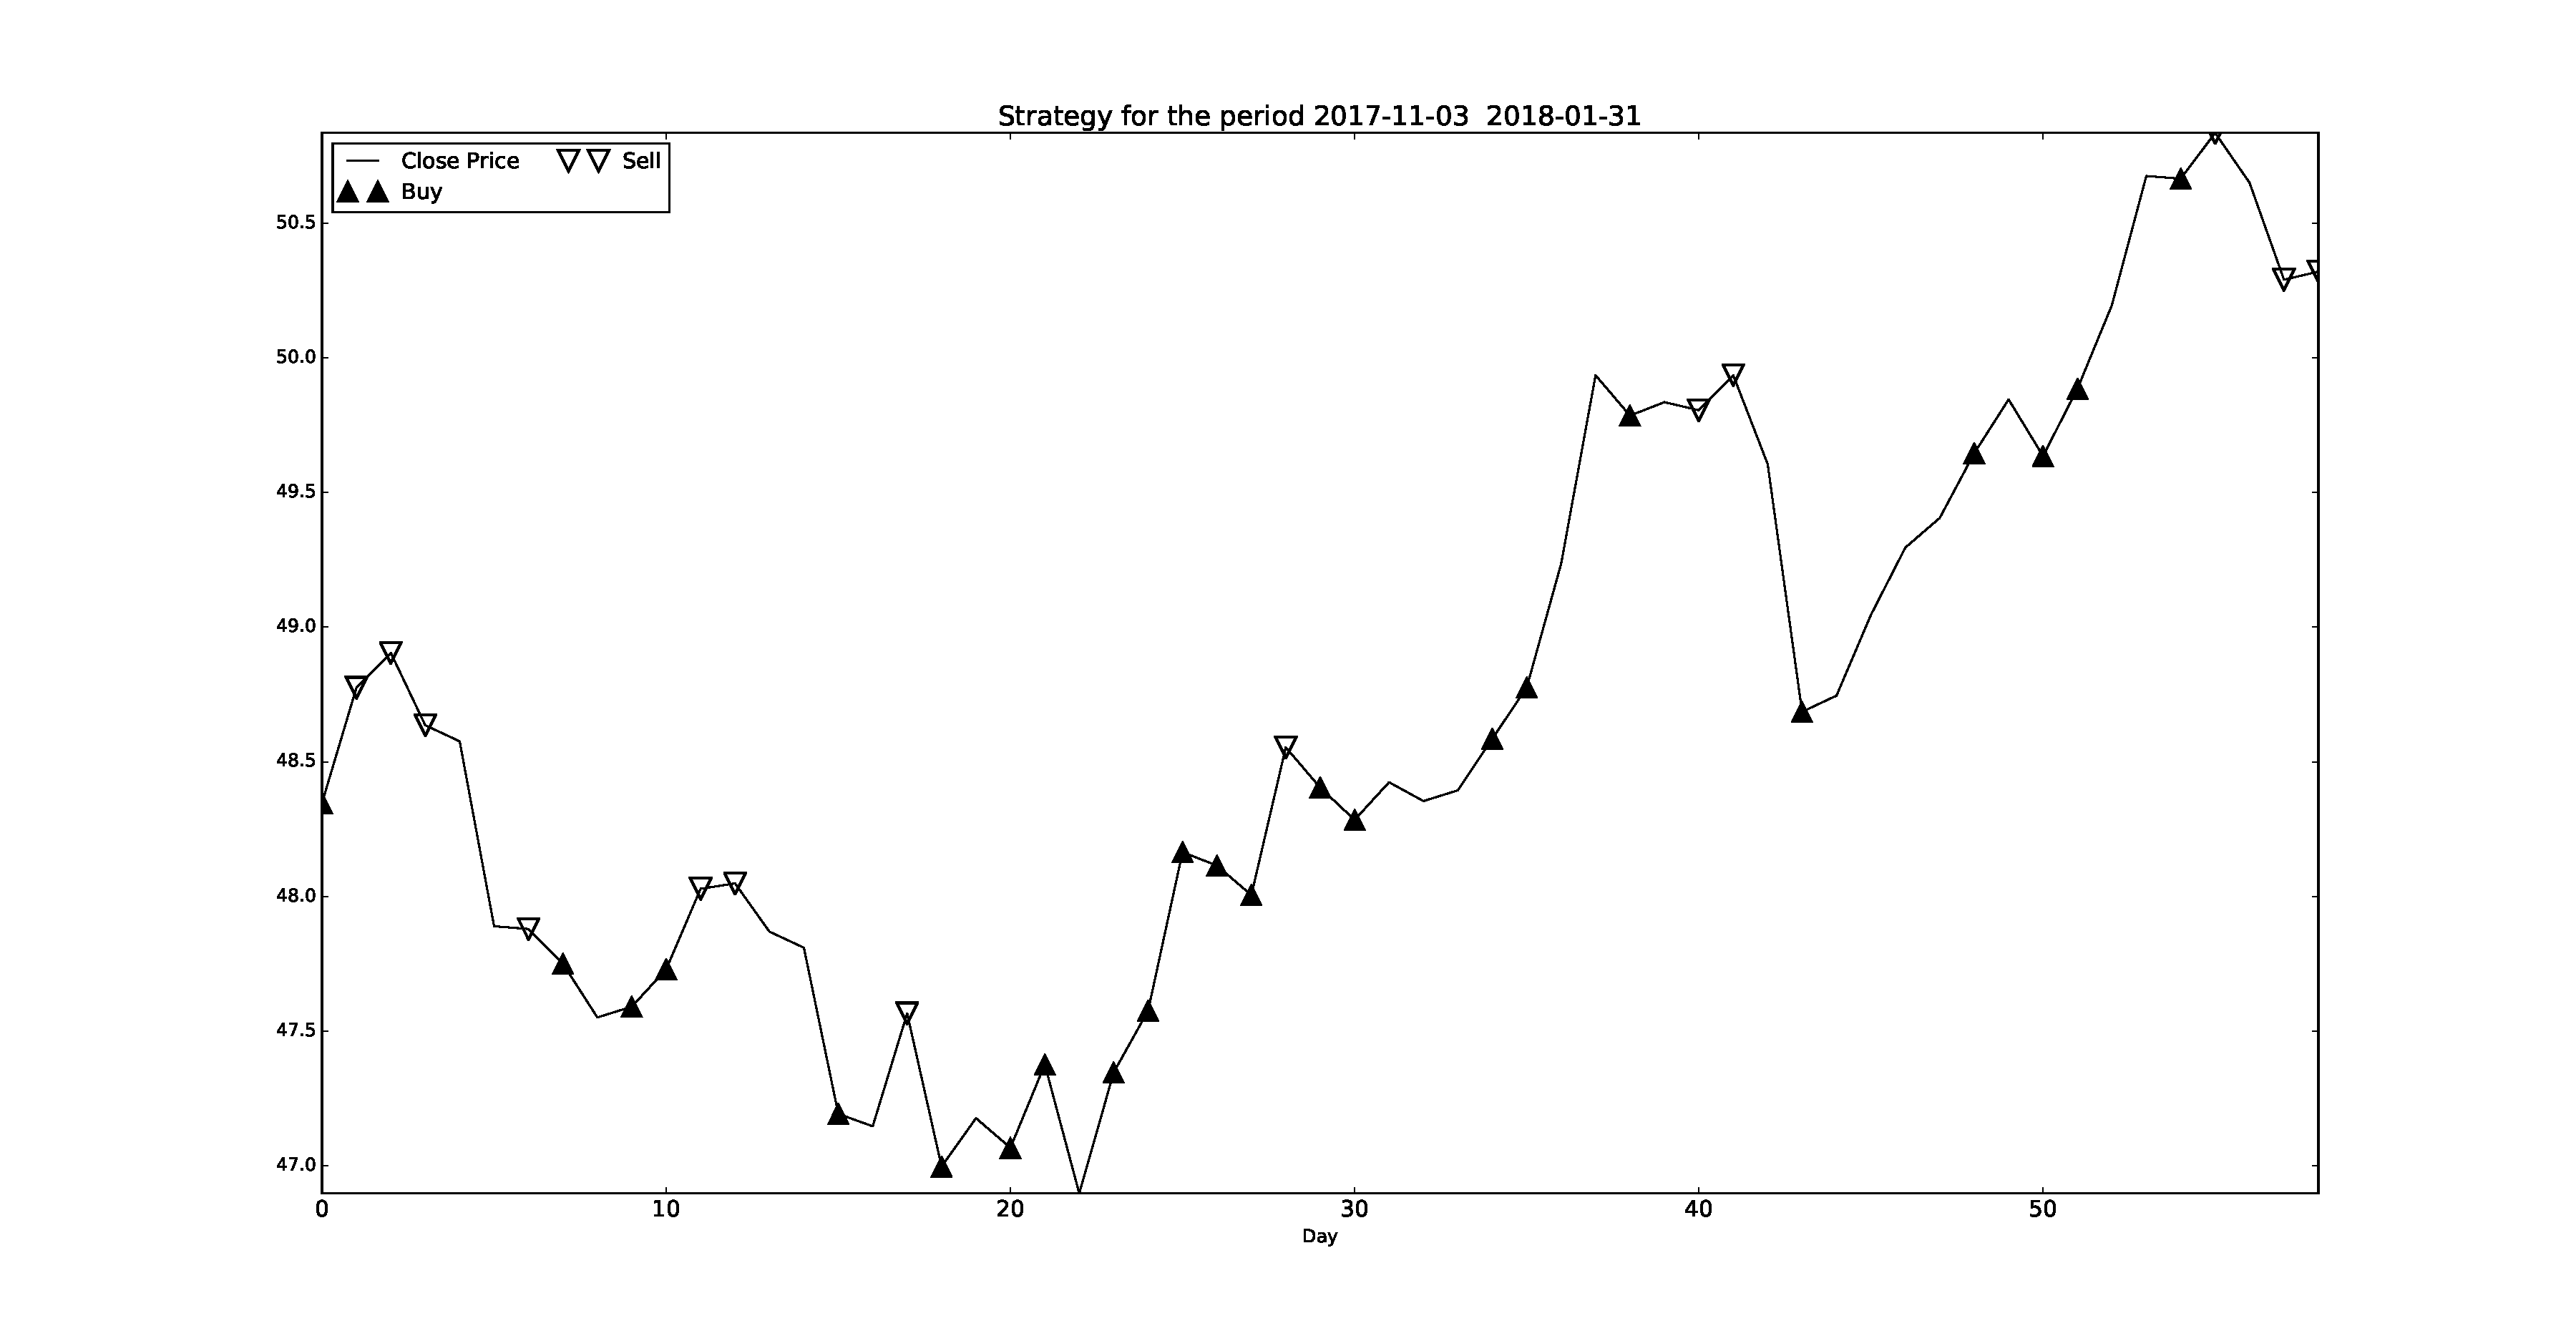
\includegraphics[width=1.0\linewidth]{imagenes/etiquetamiento_ENG}}
	\caption{Results from the labeling process}
	\label{fig:etiquetamiento}
\end{figure}

\subsection{Features}

For each day, the open, minimum, maximum and adjusted close prices were used as features.


\subsection{Results}

For every training and test set, the following models were tested\footnote{We chose these models since they're among the most popular ones used in the pattern recognition literature (see \cite{bishop} and \cite{quinlan} for their mathematical description) .
}:

\begin{itemize}

	\item Support Vector Machine with gaussian kernel and assigning class weigths of $0.45, 0.10, 0.45$ for classes $-1, 0, 1$ respectively. 
	
	\item Multilayer perceptron with a hidden layer with 10 neurons and \textit{ReLu} as activation function.
	
	
	\item C4.5 tree with max depth of 5.	
	
\end{itemize}


As described above, the performance measure was \textbf{Excess Return} which is calculated using the following assumptions:

%\subsubsection{Assumptions}
\begin{itemize}

	\item No short-sales allowed, this means that one can only sell if a buy action occurred in the past (we can't sell something that we don't own).
	
	\item Once a trading signal is activated, we have to wait until we see a different one, so no repetitions of the same signal are allowed. This avoids excessive buys or sells.
		
	\item Since we are using end of day data, if we have a buy or sell signal on day $t$, then the buy or sell price (execution price) is the average between the minimum and maximum price at day $t+1$.
	
	\item The cost of every transaction is equal to a $0.25 \%$ over the total cost. For example, if a stock was bought  at a price of $\$10$, then the actual monetary amount paid for it is equal to $\$10(1+0.0025)$; likewise if a stock was sold at a price of $\$10$ we end up receiving. a monetary amount of $\$10(1-0.0025)$.
\end{itemize}

For every test set and every model we obtained the following results.

\begin{table}[H]
\caption{Results obtained for every model}
\label{table excess returns}
\centering
\begin{tabular}{p{5cm}rrr}
	\hline
	\multicolumn{4}{r}{Excess Return} \\
	\hline
	Test set & SVM & MLP & C4.5 \\
	\hline
	2014-05-02 / 2014-07-31 & -0.013  & -0.067 & -0.067 \\
	2014-08-04 / 2014-10-31 & 0.0 & -0.006 & -0.006 \\
	2014-11-03 / 2015-01-30 & 0.0 & 0.0 & 0.0 \\
	2015-02-03 / 2015-04-30 & -0.058 &  -0.066 & -0.07 \\
	2015-05-04 / 2015-07-31 & 0.0 & 0.0 & -0.039 \\
	2015-08-03 / 2015-10-30 & 0.02 & 0.0 & 0.025 \\
	2015-11-04 / 2016-01-29 & 0.113 & 0.054 & 0.091 \\
	2016-02-02 / 2016-04-28 & -0.053 & -0.025 & -0.065 \\
	2016-05-02 / 2016-07-29 & 0.046 & -0.025 &  -0.024 \\
	2016-08-01 / 2016-10-31 & 0.003 & -0.027 & -0.027 \\
	2016-11-01 / 2017-01-31 & 0.028 & 0.004 & 0.01 \\
	2017-02-01 / 2017-04-28 & -0.008 & -0.045 & -0.047 \\
	2017-05-02 / 2017-07-31 & -0.029 & -0.029 & -0.014 \\
	2017-08-01 / 2017-10-31 & 0.016 & 0.054 & 0.045 \\
	2017-11-03 / 2018-01-31 & -0.033 & 0.032 & -0.06 \\
	2018-02-01 / 2018-04-05 & 0.0 & 0.0 &  0.069 \\
	
	\hline
	Overall sum & 0.32 & -0.174 & -0.179 \\
	
	\hline
	Average & 0.002 & -0.01 & -0.011 \\
	\hline
	Number of positive excess returns &  6 & 4 & 5 \\
	\hline
	Number of negative excess returns & 6 & 8 & 10 \\  
	

	\hline 
\end{tabular}
\end{table}	

\newpage

\section{Conclusions}

As we can observe, among the three models used, the best results were obtained by the Support Vector Machine.

Unfortunately, even tough when in this model we obtained a positive average excess return, using a t-test for the mean (with a confidence level of $95 \%$) we found that is not possible to reject the null hypothesis (the true mean is zero) thus, statistically speaking, we can't conclude that this method beats the BH strategy systematically.

Nonetheless it's worth to mention that thanks to the labeling method we can explore further other types of supervised learning techniques whether using a symbolic or sub-symbolic approach.

The future directions for this work might be:

\begin{itemize}
	\item Explore symbolic approaches for supervised learning, such as Extended Classifier System (XCS).
	\item Analyze the inclusion of technical indicators.
	\item Use another set of features.
	\item Use other sampling frequencies.
	\item Use risk-adjusted performance measures.
\end{itemize}

\newpage 
\bibliographystyle{splncs04}
\bibliography{referencias_articulo}{}



\end{document}